
TraceR-CODES has been previously validated with micro-benchmarks and stand alone
applications including pF3D, 3D Stencil, ping-pong, all-to-all,
etc~\cite{Jain:sc2017}. These validation studies were done for fat-tree networks
and it was found that TraceR-CODES predicts the absolute value as well as the
trends in the execution time with less than 15\%
error~\cite{Jain:sc2017,acun:padabs2015}.  However, these validation studies 
have been done with single job simulations. Further, these studies did not
validate cross-platform and cross-network projections, i.e. traces were
collected and projections were done for the same system.

To gain confidence in TraceR-CODES' prediction for cross-platform and
cross-network multi-job workloads as well
as in the new additions to TraceR-CODES, this work validates TraceR-CODES with three random
multi-job workloads.
The validation is done by 1)~randomly creating three workloads that consist of 
representative HPC benchmarks with different communication and computation
characteristics, 2)~running the workloads on the Quartz supercomputer~\cite{quartz} at LLNL,
3)~simulating the workloads using TraceR-CODES with the system parameters
set to the values for Quartz, and 4)~comparing the predicted job execution
times from the simulations with the measured times on Quartz. 

The three workloads are formed by selecting jobs from two communication intensive
benchmarks (Stencil4d and Subcomm3d) and two computation intensive applications
(Kripke and Laghos). 

In this study, three workloads were run in a dedicated access time (DAT) on Quartz at LLNL, during this period
no other jobs ran on the machine. It used linear mapping of job
ranks to nodes and measured the execution time of each job in the workloads.
For simulation with the TraceR-CODES framework, it used the
exact system settings as Quartz: (1)  create
the exact fat-tree topology as Quartz using the arbitrary graph model; (2)
 set the values of the network parameters to the corresponding values on Quartz:
11.9 GB/s peak link bandwidth, 8 packets buffer size, 4096 bytes packet size,
and so on; and (3) the jobs and processes in each workload
are mapped to compute nodes exactly in the same
way as they ran on Quartz. 

The traces for driving the simulation were collected on
Vulcan~\cite{vulcan}, a 5D-torus based Blue Gene/Q
system.  Since the computational capabilities of Vulcan are different from
Quartz, the relative compute scaling factor between Vulcan and
Quartz is calculated, and the computation regions of simulations were scaled accordingly. This
setup helps to evaluate the projections when the network (5D-torus vs fat-tree)
as well as computational capability (IBM PowerPC vs Intel Xeon) of the traced
system are different from the target system.
%Finally, I use the exact job and node mapping in the simulation as the real
%job when run on Quartz. 
\FloatBarrier
\begin{figure}[!htbp]
  \centering
  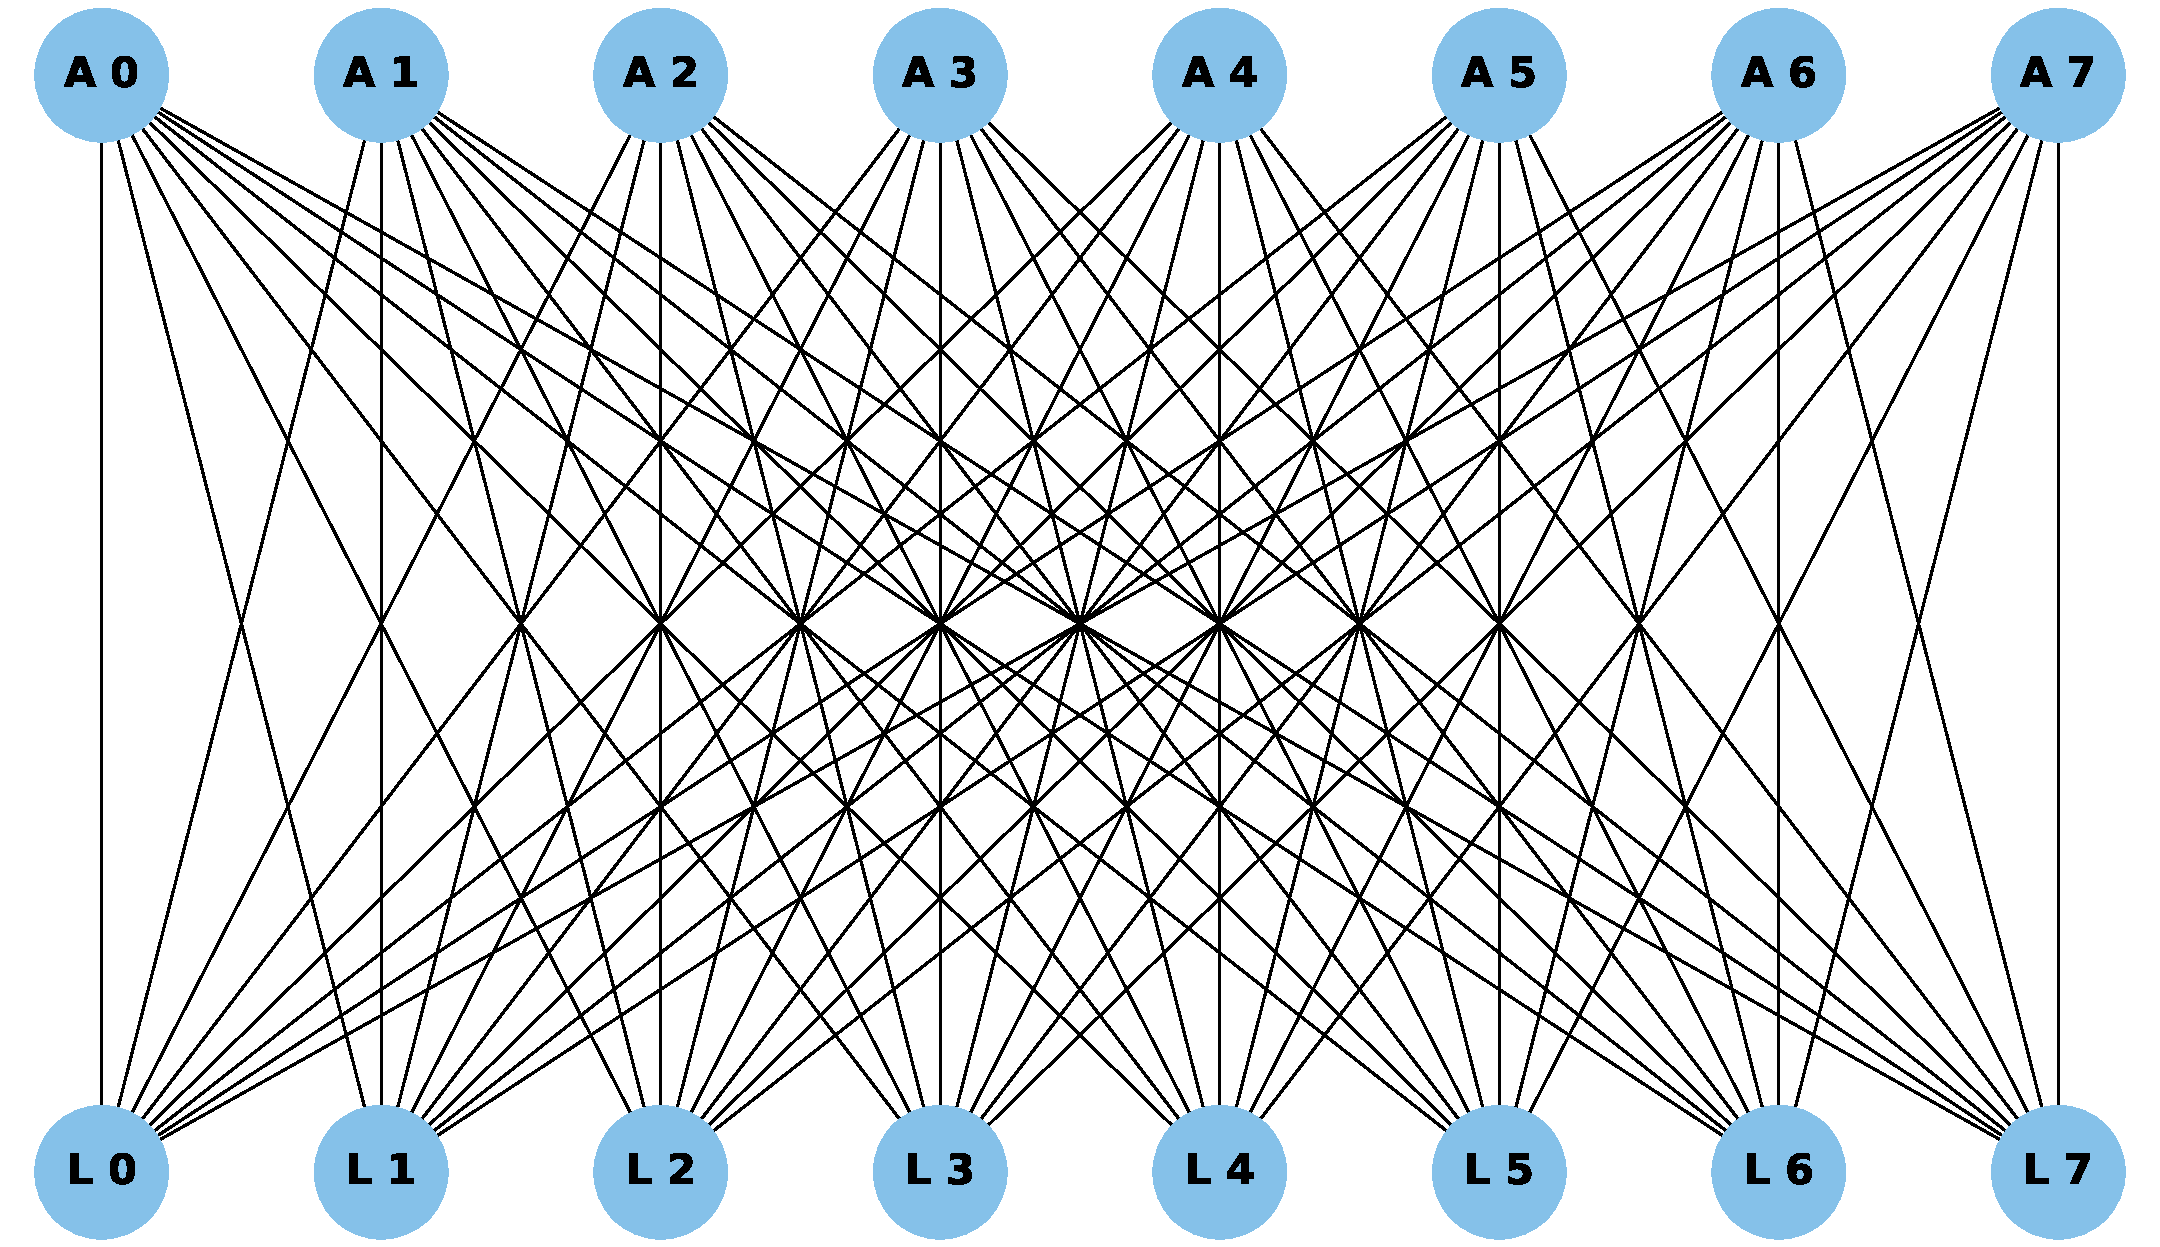
\includegraphics[width=0.8\columnwidth]{figure/val/quartztopo.pdf}
  \caption{A Quartz pod with eight aggregate and eight leaf switches, and all links.}
  \label{fig:quartz_pod}
%\end{multicols}
\end{figure}
\FloatBarrier
\vspace{0.08in}
\noindent{\bf Quartz Topology:} The Quartz system deploys a 3-level fat-tree, with a 2:1
tapering at each of its 84 leaf switches. There are 84 aggregate switches and 32
core switches. Each switch has a radix of 48 and each leaf level switch is
connected to 32 compute nodes.  Note that some ports in the aggregate switches
and core switches are left unused.  The 84 leaf level switches are divided among 
11 pods. Figure~\ref{fig:quartz_pod} shows a Quartz supercomputer pod.  Each pod consists 
of 8 leaf switches and 8 aggregate switches, which are connected in an
all-to-all bipartite graph. Each arc drawn here represents two physical links. 
In contrast, a standard 2:1 tapered fat-tree would have 16 leaf switches in 
each pod, which are connected to 16 aggregate switches using one physical link
each. We give these details of the Quartz topology to highlight that
Quartz' fat-tree is different from the standard, symmetric fat-tree topology,
as are the networks in most production systems. These differences are the main driver
for the development of the {\em arbitrary graph model}. 

Figure~\ref{fig:validation} shows the results of the validation. The
horizontal axis, have each application and their corresponding job size used
in various workloads. Each blue dot represents the average 
of the error percentage between the predicted runtime and the measured runtime
for various
instances of the given application-job size pair that appear across the three workloads. For
example, since Subcomm3d jobs with a process count of 128 appears two times
across the three workloads, their average error percentage is computed to be
-7.88\%. It can be observed, that for all cases except 32-ranks
Stencil4d, the prediction error is within 20\%; and for all except 3 cases
(32-rank Stencil4d, 32-ranks Kripke, and 64-ranks Kripke), the error is within 15\%.
These results suggest that TraceR-CODES predictions reasonably approximate 
the actual runtime on real systems for multi-job workloads even when the
computational capability and underlying network are different.

\begin{figure}[!htbp]
\centering
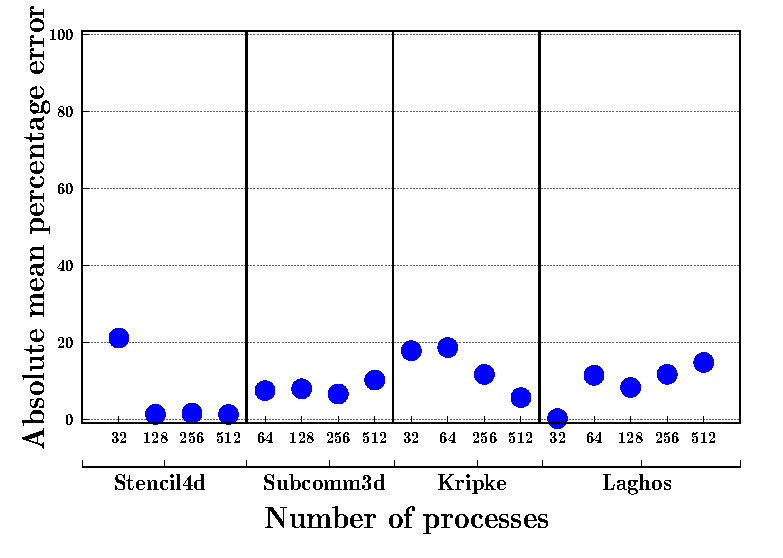
\includegraphics[width=\columnwidth]{figure/val/quartz.eps}
\caption{Validation of TraceR-CODES (mean percentage error in predicted runtime compared to the actual runtime).}
\label{fig:validation}
\end{figure}

